% 若编译失败,且生成 .synctex(busy) 辅助文件,可能有两个原因:
% 1. 需要插入的图片不存在:Ctrl + F 搜索 'figure' 将这些代码注释/删除掉即可
% 2. 路径/文件名含中文或空格:更改路径/文件名即可

% --------------------- 文章宏包及相关设置 --------------------- %
% >> ------------------ 文章宏包及相关设置 ------------------ << %
% 设定文章类型与编码格式
\documentclass[UTF8]{article}		

% 物理实验报告所需的其它宏包
\usepackage{ulem}   % \uline 下划线支持
\usepackage{circuitikz} % 电路图 tikz 支持
\usepackage{pdfpages}   % 用于导入 pdf 文件

% 本 .tex 专属的宏定义
    \def\V{\ \mathrm{V}}
    \def\uV{\ \mu\mathrm{V}}
    \def\mV{\ \mathrm{mV}}
    \def\K{\ \mathrm{K}}
    \def\kV{\ \mathrm{KV}}
    \def\KV{\ \mathrm{KV}}
    \def\MV{\ \mathrm{MV}}
    \def\uA{\ \mu\mathrm{A}}
    \def\mA{\ \mathrm{mA}}
    \def\A{\ \mathrm{A}}
    \def\kA{\ \mathrm{KA}}
    \def\KA{\ \mathrm{KA}}
    \def\MA{\ \mathrm{MA}}
    \def\O{\ \Omega}
    \def\mO{\ \Omega}
    \def\kO{\ \mathrm{K}\Omega}
    \def\KO{\ \mathrm{K}\Omega}
    \def\MO{\ \mathrm{M}\Omega}
    \def\Hz{\ \mathrm{Hz}}
    \def\uF{\ \mu\mathrm{F}}
    \def\mF{\ \mathrm{mF}}
    \def\F{\ \mathrm{F}}
    \def\Re{\mathrm{\,Re}\,}
    \def\Im{\mathrm{\,Im}\,}
    \def\sinc{\mathrm{\,sinc}\,}

% 自定义宏定义
    \def\N{\mathbb{N}}
    \def\F{\mathbb{F}}
    \def\Z{\mathbb{Z}}
    \def\Q{\mathbb{Q}}
    \def\R{\mathbb{R}}
    \def\C{\mathbb{C}}
    \def\T{\mathbb{T}}
    \def\S{\mathbb{S}}
    %\def\A{\mathbb{A}}
    \def\I{\mathscr{I}}
    \def\d{\mathrm{d}}
    \def\p{\partial}


% 导入基本宏包
    \usepackage[UTF8]{ctex}     % 设置文档为中文语言
    \usepackage{hyperref}  % 宏包:自动生成超链接 (此宏包与标题中的数学环境冲突)
    \hypersetup{
        colorlinks=true,    % false:边框链接 ; true:彩色链接
        citecolor={blue},    % 文献引用颜色
        linkcolor={blue},   % 目录 (我们在目录处单独设置),公式,图表,脚注等内部链接颜色
        urlcolor={magenta},    % 网页 URL 链接颜色,包括 \href 中的 text
        % cyan 浅蓝色 
        % magenta 洋红色
        % yellow 黄色
        % black 黑色
        % white 白色
        % red 红色
        % green 绿色
        % blue 蓝色
        % gray 灰色
        % darkgray 深灰色
        % lightgray 浅灰色
        % brown 棕色
        % lime 石灰色
        % olive 橄榄色
        % orange 橙色
        % pink 粉红色
        % purple 紫色
        % teal 蓝绿色
        % violet 紫罗兰色
    }
    % \usepackage{docmute}    % 宏包:子文件导入时自动去除导言区,用于主/子文件的写作方式,\include{./51单片机笔记}即可。注:启用此宏包会导致.tex文件capacity受限。
    \usepackage{amsmath}    % 宏包:数学公式
    \usepackage{mathrsfs}   % 宏包:提供更多数学符号
    \usepackage{amssymb}    % 宏包:提供更多数学符号
    \usepackage{pifont}     % 宏包:提供了特殊符号和字体
    \usepackage{extarrows}  % 宏包:更多箭头符号 
    \usepackage{multicol}   % 宏包:支持多栏 

% 文章页面margin设置
    \usepackage[a4paper]{geometry}
        \geometry{top=0.75in}
        \geometry{bottom=0.75in}
        \geometry{left=0.75in}
        \geometry{right=0.75in}   % 设置上下左右页边距
        \geometry{marginparwidth=1.75cm}    % 设置边注距离(注释、标记等)

% 配置数学环境
    \usepackage{amsthm} % 宏包:数学环境配置
    % theorem-line 环境自定义
        \newtheoremstyle{MyLineTheoremStyle}% <name>
            {11pt}% <space above>
            {11pt}% <space below>
            {\kaishu}% <body font> 默认使用正文字体, \kaishu 为楷体
            {}% <indent amount>
            {\bfseries}% <theorem head font> 设置标题项为加粗
            {:\ \ }% <punctuation after theorem head>
            {.5em}% <space after theorem head>
            {\textbf{#1}\thmnumber{#2}\ \ (\,\textbf{#3}\,)}% 设置标题内容顺序
        \theoremstyle{MyLineTheoremStyle} % 应用自定义的定理样式
        \newtheorem{LineTheorem}{Theorem.\,}
    % theorem-block 环境自定义
        \newtheoremstyle{MyBlockTheoremStyle}% <name>
            {11pt}% <space above>
            {11pt}% <space below>
            {\kaishu}% <body font> 使用默认正文字体
            {}% <indent amount>
            {\bfseries}% <theorem head font> 设置标题项为加粗
            {:\\ \indent}% <punctuation after theorem head>
            {.5em}% <space after theorem head>
            {\textbf{#1}\thmnumber{#2}\ \ (\,\textbf{#3}\,)}% 设置标题内容顺序
        \theoremstyle{MyBlockTheoremStyle} % 应用自定义的定理样式
        \newtheorem{BlockTheorem}[LineTheorem]{Theorem.\,} % 使用 LineTheorem 的计数器
    % definition 环境自定义
        \newtheoremstyle{MySubsubsectionStyle}% <name>
            {11pt}% <space above>
            {11pt}% <space below>
            {}% <body font> 使用默认正文字体
            {}% <indent amount>
            {\bfseries}% <theorem head font> 设置标题项为加粗
            {:\\ \indent}% <punctuation after theorem head>
            {0pt}% <space after theorem head>
            {\textbf{#3}}% 设置标题内容顺序
        \theoremstyle{MySubsubsectionStyle} % 应用自定义的定理样式
        \newtheorem{definition}{}

%宏包:有色文本框(proof环境)及其设置
\usepackage{xcolor}    %设置插入的文本框颜色
    % rgb(4, 9, 103), rgb(5, 13, 164)
    % rgb(124, 131, 255), rgb(231, 232, 255)
    % rgb(255, 190, 190), rgb(255, 70, 70)
    \definecolor{stc}{RGB}{4, 10, 118}  % 设置各级标题结构颜色
\usepackage[strict]{changepage}     % 提供一个 adjustwidth 环境
\usepackage{framed}     % 实现方框效果
    % rgb(0, 0, 0), rgb(100, 100, 100)
    %#ECECED 为 0.93, 0.93, 0.93
    \definecolor{graybox_color}{rgb}{0.93, 0.93, 0.93} % 这里的 rbg 范围是 [0, 1]
    % 文本框颜色。修改此行中的 rgb 数值即可改变方框纹颜色,具体颜色的rgb数值可以在网站https://colordrop.io/ 中获得。(截止目前的尝试还没有成功过,感觉单位不一样)(找到喜欢的颜色,点击下方的小眼睛,找到rgb值,复制修改即可)
    \newenvironment{graybox}{%
    \def\FrameCommand{%
    \hspace{1pt}%
    {\color{gray}\small \vrule width 2pt}%
    {\color{graybox_color}\vrule width 4pt}%
    \colorbox{graybox_color}%
    }%
    \MakeFramed{\advance\hsize-\width\FrameRestore}%
    \noindent\hspace{-4.55pt}% disable indenting first paragraph
    \begin{adjustwidth}{}{7pt}%
    \vspace{2pt}\vspace{2pt}%
    }
    {%
    \vspace{2pt}\end{adjustwidth}\endMakeFramed%
    }

    \definecolor{bluebox_ruleColor}{rgb}{0.49, 0.51, 1} % 文本框颜色。修改此行中的 rgb 数值即可改变方框纹颜色,具体颜色的rgb数值可以在网站https://colordrop.io/ 中获得。(截止目前的尝试还没有成功过,感觉单位不一样)(找到喜欢的颜色,点击下方的小眼睛,找到rgb值,复制修改即可)
    \definecolor{bluebox_backgroundColor}{rgb}{0.93, 0.93, 1}
    \newenvironment{bluebox}{%
    \def\FrameCommand{%
    \hspace{1pt}%
    {\color{bluebox_ruleColor}\small \vrule width 2pt}%
    {\color{bluebox_backgroundColor}\vrule width 4pt}% 4pt 缩进比较合适
    \colorbox{bluebox_backgroundColor}%
    }%
    \MakeFramed{\advance\hsize-\width\FrameRestore}%
    \noindent\hspace{-4.55pt}% disable indenting first paragraph
    \begin{adjustwidth}{}{7pt}%
    \vspace{2pt}\vspace{2pt}%
    }
    {%
    \vspace{2pt}\end{adjustwidth}\endMakeFramed%
    }

    \definecolor{redbox_ruleColor}{rgb}{1, 0.27, 0.27} % 文本框颜色。修改此行中的 rgb 数值即可改变方框纹颜色,具体颜色的rgb数值可以在网站https://colordrop.io/ 中获得。(截止目前的尝试还没有成功过,感觉单位不一样)(找到喜欢的颜色,点击下方的小眼睛,找到rgb值,复制修改即可)
    \definecolor{redbox_backgroundColor}{rgb}{1, 0.90, 0.90}
    \newenvironment{redbox}{%
    \def\FrameCommand{%
    \hspace{1pt}%
    {\color{redbox_ruleColor}\small \vrule width 2pt}%
    {\color{redbox_backgroundColor}\vrule width 4pt}% 4pt 缩进比较合适
    \colorbox{redbox_backgroundColor}%
    }%
    \MakeFramed{\advance\hsize-\width\FrameRestore}%
    \noindent\hspace{-4.55pt}% disable indenting first paragraph
    \begin{adjustwidth}{}{7pt}%
    \vspace{2pt}\vspace{2pt}%
    }
    {%
    \vspace{2pt}\end{adjustwidth}\endMakeFramed%
    }

% 外源代码插入设置
    % matlab 代码插入设置
    \usepackage{matlab-prettifier}
        \lstset{style=Matlab-editor}    % 继承 matlab 代码高亮 , 此行不能删去
    \usepackage[most]{tcolorbox} % 引入tcolorbox包 
    \usepackage{listings} % 引入listings包
        \tcbuselibrary{listings, skins, breakable}
        \newfontfamily\codefont{Consolas} % 定义需要的 codefont 字体
        \lstdefinestyle{MatlabStyle_inc}{   % 插入代码的样式
            language=Matlab,
            basicstyle=\footnotesize\ttfamily\codefont,    % ttfamily 确保等宽 
            breakatwhitespace=false,
            breaklines=true,
            captionpos=b,
            keepspaces=true,
            numbers=left,
            numbersep=15pt,
            showspaces=false,
            showstringspaces=false,
            showtabs=false,
            tabsize=2,
            xleftmargin=15pt,   % 左边距
            %frame=single, % single 为包围式单线框
            frame=shadowbox,    % shadowbox 为带阴影包围式单线框效果
            %escapeinside=``,   % 允许在代码块中使用 LaTeX 命令 (此行无用)
            %frameround=tttt,    % tttt 表示四个角都是圆角
            framextopmargin=0pt,    % 边框上边距
            framexbottommargin=0pt, % 边框下边距
            framexleftmargin=5pt,   % 边框左边距
            framexrightmargin=5pt,  % 边框右边距
            rulesepcolor=\color{red!20!green!20!blue!20}, % 阴影框颜色设置
            %backgroundcolor=\color{blue!10}, % 背景颜色
        }
        \lstdefinestyle{MatlabStyle_src}{   % 插入代码的样式
            language=Matlab,
            basicstyle=\small\ttfamily\codefont,    % ttfamily 确保等宽 
            breakatwhitespace=false,
            breaklines=true,
            captionpos=b,
            keepspaces=true,
            numbers=left,
            numbersep=15pt,
            showspaces=false,
            showstringspaces=false,
            showtabs=false,
            tabsize=2,
        }
        \newtcblisting{matlablisting}{
            %arc=2pt,        % 圆角半径
            % 调整代码在 listing 中的位置以和引入文件时的格式相同
            top=0pt,
            bottom=0pt,
            left=-5pt,
            right=-5pt,
            listing only,   % 此句不能删去
            listing style=MatlabStyle_src,
            breakable,
            colback=white,   % 选一个合适的颜色
            colframe=black!0,   % 感叹号后跟不透明度 (为 0 时完全透明)
        }
        \lstset{
            style=MatlabStyle_inc,
        }

% table 支持
    \usepackage{booktabs}   % 宏包:三线表
    \usepackage{tabularray} % 宏包:表格排版
    \usepackage{longtable}  % 宏包:长表格

% figure 设置
    \usepackage{graphicx}  % 支持 jpg, png, eps, pdf 图片 
    \usepackage{svg}       % 支持 svg 图片
        \svgsetup{
            % 指向 inkscape.exe 的路径
            inkscapeexe = C:/aa_MySame/inkscape/bin/inkscape.exe, 
            % 一定程度上修复导入后图片文字溢出几何图形的问题
            inkscapelatex = false                 
        }
    \usepackage{subcaption} % 用于子图和小图注  

% 图表进阶设置
    \usepackage{caption}    % 图注、表注
        \captionsetup[figure]{name=图}  
        \captionsetup[table]{name=表}
        \captionsetup{
            labelfont=bf, % 设置标签为粗体
            textfont=bf,  % 设置文本为粗体
            font=small  
        }
    \usepackage{float}     % 图表位置浮动设置 
    \usepackage{etoolbox} % 用于保证图注表注的数学字符为粗体
        \AtBeginEnvironment{figure}{\boldmath} % 图注中的数学字符为粗体
        \AtBeginEnvironment{table}{\boldmath}  % 表注中的数学字符为粗体
        \AtBeginEnvironment{tabular}{\unboldmath}   % 保证表格中的数学字符不受额外影响

% 圆圈序号自定义
    \newcommand*\circled[1]{\tikz[baseline=(char.base)]{\node[shape=circle,draw,inner sep=0.8pt, line width = 0.03em] (char) {\bfseries #1};}}   % TikZ solution

% 列表设置
    \usepackage{enumitem}   % 宏包:列表环境设置
        \setlist[enumerate]{
            label=(\arabic*) ,   % 设置序号样式为加粗的 (1) (2) (3)
            ref=\arabic*, % 如果需要引用列表项,这将决定引用格式(这里仍然使用数字)
            itemsep=0pt, parsep=0pt, topsep=0pt, partopsep=0pt, leftmargin=3.5em} 
        \setlist[itemize]{itemsep=0pt, parsep=0pt, topsep=0pt, partopsep=0pt, leftmargin=3.5em}
        \newlist{circledenum}{enumerate}{1} % 创建一个新的枚举环境  
        \setlist[circledenum,1]{  
            label=\protect\circled{\arabic*}, % 使用 \arabic* 来获取当前枚举计数器的值,并用 \circled 包装它  
            ref=\arabic*, % 如果需要引用列表项,这将决定引用格式(这里仍然使用数字)
            itemsep=0pt, parsep=0pt, topsep=0pt, partopsep=0pt, leftmargin=3.5em
        }  

% 其它设置
    % 脚注设置
        \renewcommand\thefootnote{\ding{\numexpr171+\value{footnote}}}
    % 参考文献引用设置
        \bibliographystyle{unsrt}   % 设置参考文献引用格式为unsrt
        \newcommand{\upcite}[1]{\textsuperscript{\cite{#1}}}     % 自定义上角标式引用
    % 文章序言设置
        \newcommand{\cnabstractname}{序言}
        \newenvironment{cnabstract}{%
            \par\Large
            \noindent\mbox{}\hfill{\bfseries \cnabstractname}\hfill\mbox{}\par
            \vskip 2.5ex
            }{\par\vskip 2.5ex}

% 文章默认字体设置
    \usepackage{fontspec}   % 宏包:字体设置
        \setmainfont{SimSun}    % 设置中文字体为宋体字体
        \setCJKmainfont[AutoFakeBold=3]{SimSun} % 设置加粗字体为 SimSun 族,AutoFakeBold 可以调整字体粗细
        \setmainfont{Times New Roman} % 设置英文字体为Times New Roman

% 各级标题自定义设置
    \usepackage{titlesec}   
        % section标题自定义设置 
        \titleformat{\section}[hang]{\normalfont\Large\bfseries\boldmath}{\thesection}{8pt}{}
        % subsection 标题自定义设置
        \titleformat{\subsection}[hang]{\normalfont\large\bfseries\boldmath}{\thesubsection}{8pt}{}
        \titlespacing*{\subsection}{0pt}{10pt}{6pt} % 控制上下间距


% --------------------- 文章宏包及相关设置 --------------------- %
% >> ------------------ 文章宏包及相关设置 ------------------ << %




% ------------------------ 文章信息区 ------------------------ %
% ------------------------ 文章信息区 ------------------------ %
% 页眉页脚设置
\usepackage{fancyhdr}   %宏包:页眉页脚设置
    \pagestyle{fancy}
    \fancyhf{}
    \cfoot{\thepage}
    \renewcommand\headrulewidth{1pt}
    \renewcommand\footrulewidth{0pt}
    %\rhead{《线性电路实验》实验报告}    
    \lhead{\small \faGithub\ \href{https://github.com/YiDingg/UCAS-LinearCircuitExperiment}{\color{black} https://github.com/YiDingg/UCAS-LinearCircuitExperiment}}


    \graphicspath{{../}}   % 修改主文件图像路径,使得子文件能够直接使用相对路径,而不是从 assets 开始索引

    \usepackage{fontawesome}    % 宏包:更多符号与图标 (用于插入 GitHub 图标等)



%%%%%%%%%%%%%%%%%%%%%%%%%%%%%%%%%%%%%%%%%%%%%%%%%%%%%%%%%%%%%%%%
% 仅需修改页眉、实验名称、实验日期
%%%%%%%%%%%%%%%%%%%%%%%%%%%%%%%%%%%%%%%%%%%%%%%%%%%%%%%%%%%%%%%%


%%%%%%%%%%%%%%%%%% 1. 修改页眉内容 %%%%%%%%%%%%%%%%%%
\rhead{Preview Report of LCE-02 三极管 (2025.04.11, 丁毅)}

% 开始编辑文章
\begin{document}
\begin{center}\large
    \vspace*{-0.8cm}
    \noindent{\huge\bfseries《\ \ 线\ \ 性\ \ 电\ \ 路\ \ 实\ \ 验\ \ \ 》\ \ 预\ \ 习\ \ 报\ \ 告 }
    \\\vspace{0.1cm}
    \noindent{
    {\bfseries 
%
%%%%%%%%%%%%%%%%%% 2. 修改实验名称 %%%%%%%%%%%%%%%%%%
    实验名称:\uline{\hspace{2.2cm} 三极管 \hspace{2.2cm}}
%
    }\hspace{0.4cm}
    指导教师:\uline{\hspace{0.8cm}王东雷\ \ \ \  \ df4dac@sina.com     \hspace{0.8cm}}
    }
    \\\vspace{0.1cm}
    \noindent
    {
    姓名:\uline{\,\,\,丁毅\,\,\,}\hspace{0.2cm}
    学号:\uline{\,\,\,{ 2023K8009908031}\,\,\,}\hspace{0.2cm}
    班级/专业:\uline{\,\,\,{2308/电子信息}\,\,\,}\hspace{0.2cm}
    分组序号:\uline{\,\,\,{2-06}\,\,\,}
    }
    \\\vspace{0.1cm}
    \noindent{
%
%%%%%%%%%%%%%%%%%% 3. 修改实验日期 %%%%%%%%%%%%%%%%%%
    实验日期:\uline{\,\,{2025.04.11}\,\,}\hspace{0.2cm}
%
    实验地点:\uline{\,\,\,教学楼{ 607}\,\,\,}\hspace{0.2cm}
    是否调课/补课:\uline{\hspace{0.26cm}否 \hspace{0.26cm}}\hspace{0.2cm}
    成绩:\uline{\hspace{2cm}}
    }
\end{center}
\vspace{-0.4cm}
\noindent\rule{\textwidth}{0.075em}   % 分割线
\vspace{-1.0cm}


% ------------------------ 文章信息区 ------------------------ %
% ------------------------ 文章信息区 ------------------------ %



%%%%%%%%%%%%%%%%%%%%%%%%%%%%%%%%%%%%%%%%%%%%%%%%%%%%%%%%%%%%%%%%%%%%%%%%%%%%%%%%%
%%%%%%%%%%%%%%%%%%%%%%%%%%%%%%%%% 下面是正文内容 %%%%%%%%%%%%%%%%%%%%%%%%%%%%%%%%%
%%%%%%%%%%%%%%%%%%%%%%%%%%%%%%%%%%%%%%%%%%%%%%%%%%%%%%%%%%%%%%%%%%%%%%%%%%%%%%%%%

\section{Electrical Characteristics pf NPN Transistor SS8050 (宏嘉诚)}

\vspace*{-6mm}
\begin{figure}[H]\centering
    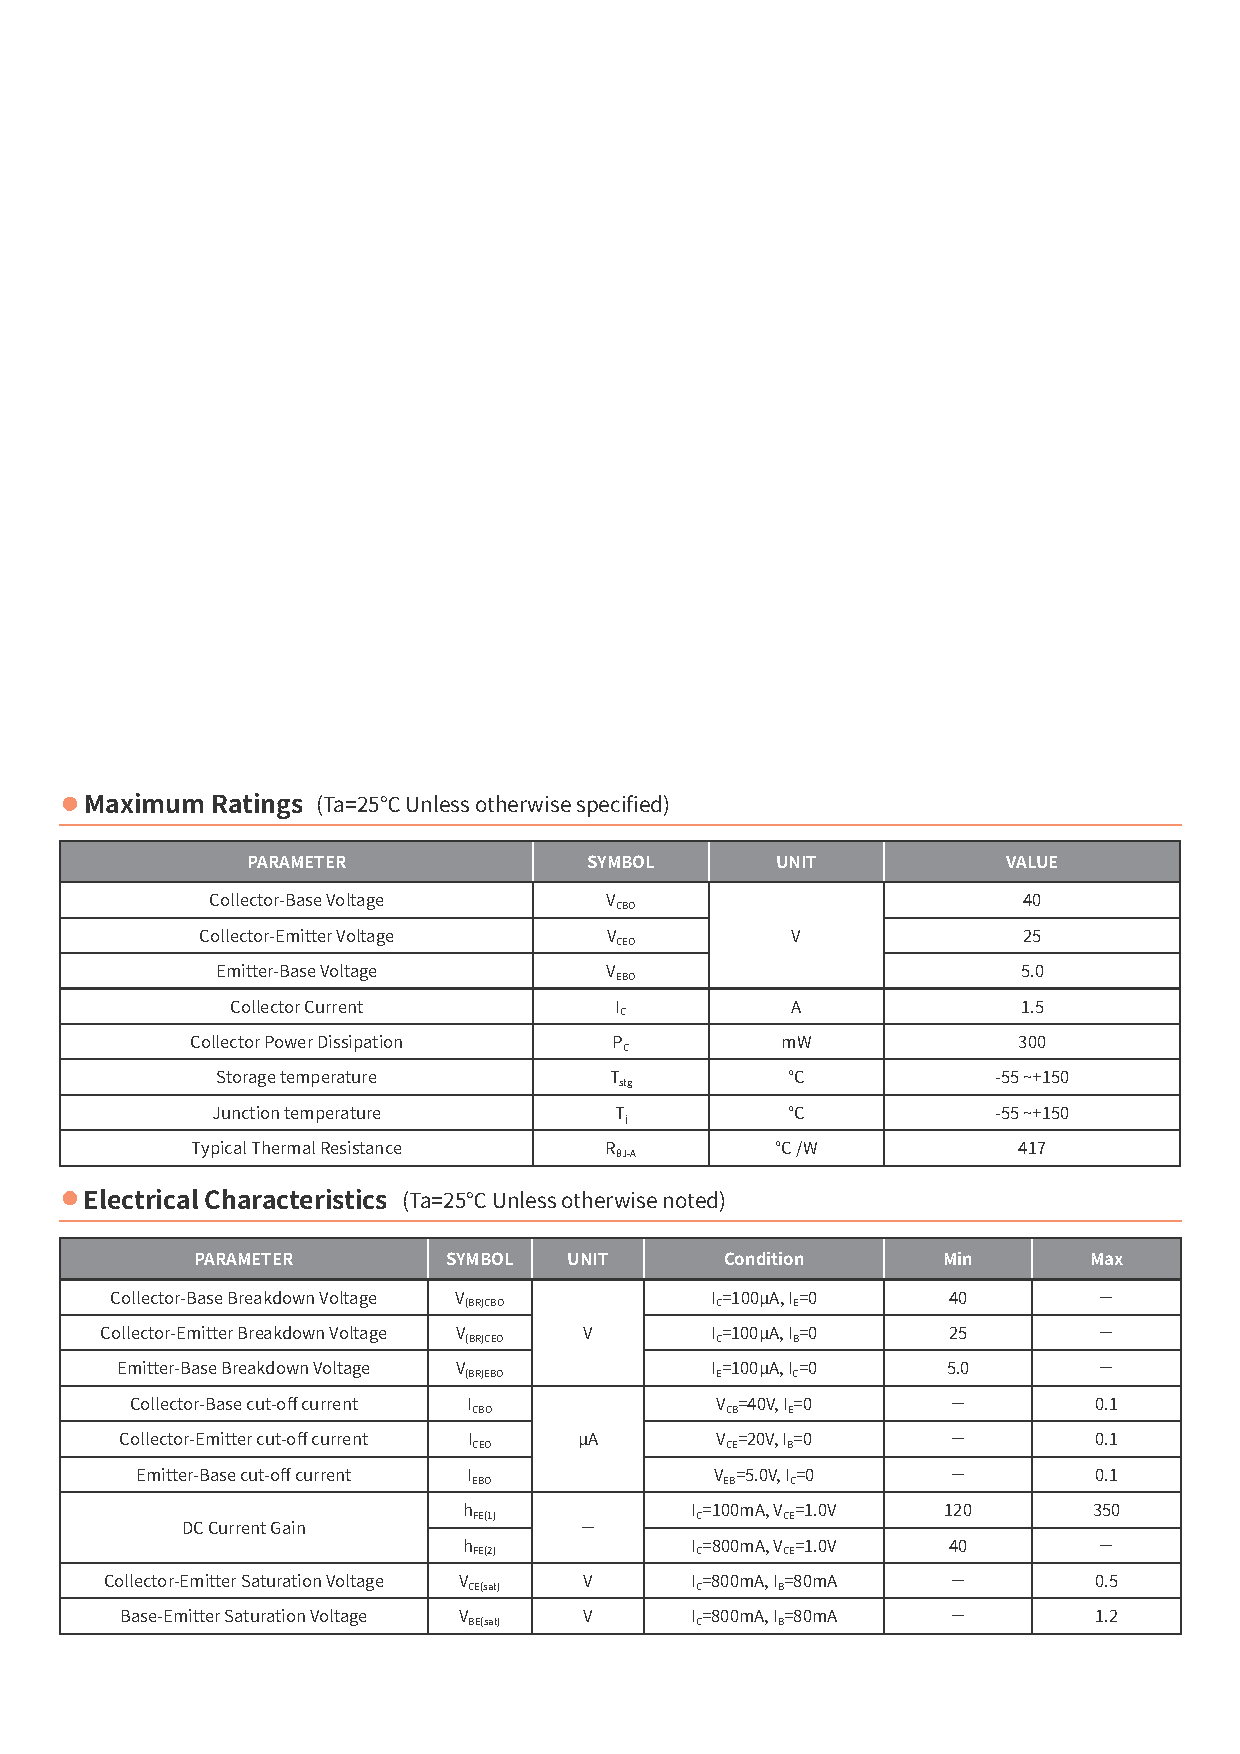
\includegraphics[width=\columnwidth]{preview/assets/SS8050_1.pdf}
    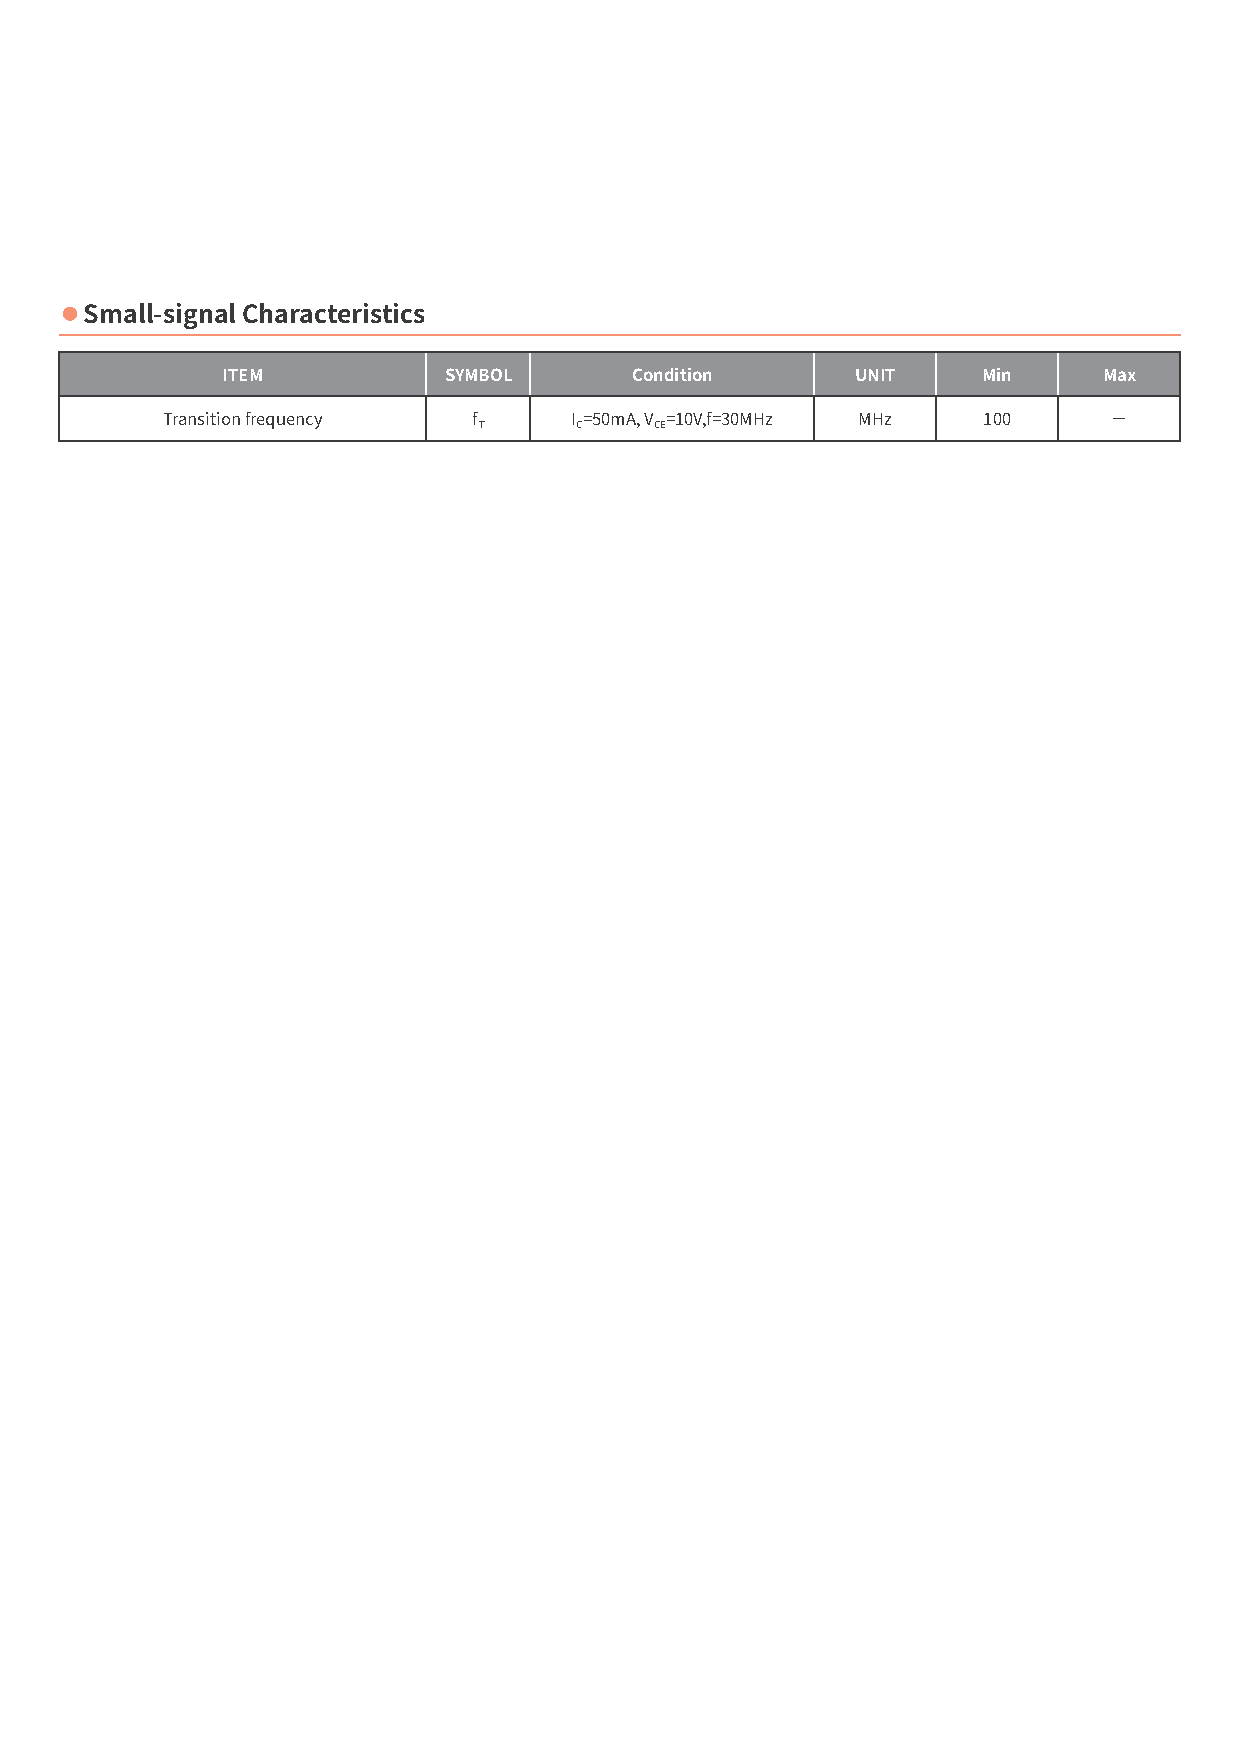
\includegraphics[width=\columnwidth]{preview/assets/SS8050_2.pdf}
\end{figure}\vspace*{-5mm}
\begin{figure}[H]\centering
    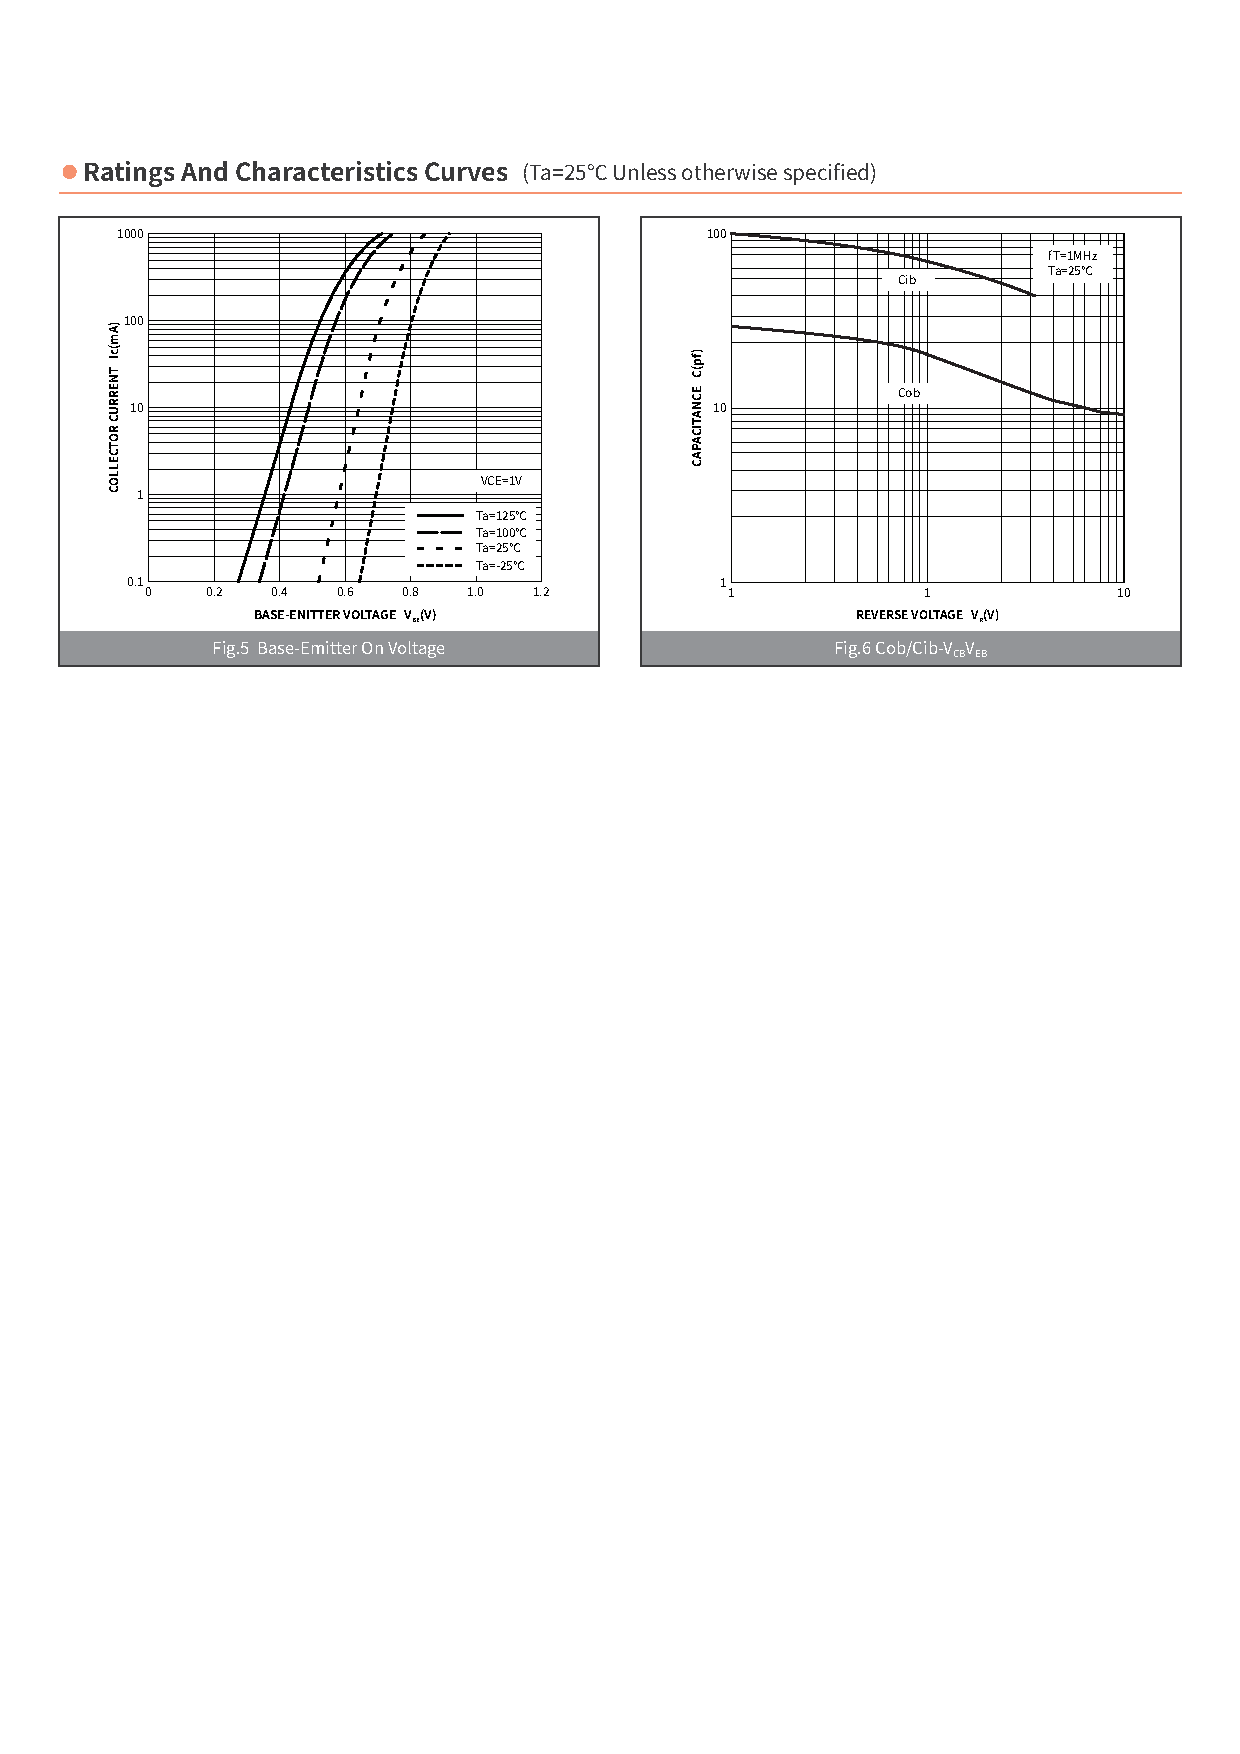
\includegraphics[width=\columnwidth]{preview/assets/SS8050_4.pdf}
\end{figure}
\begin{figure}[H]\centering
    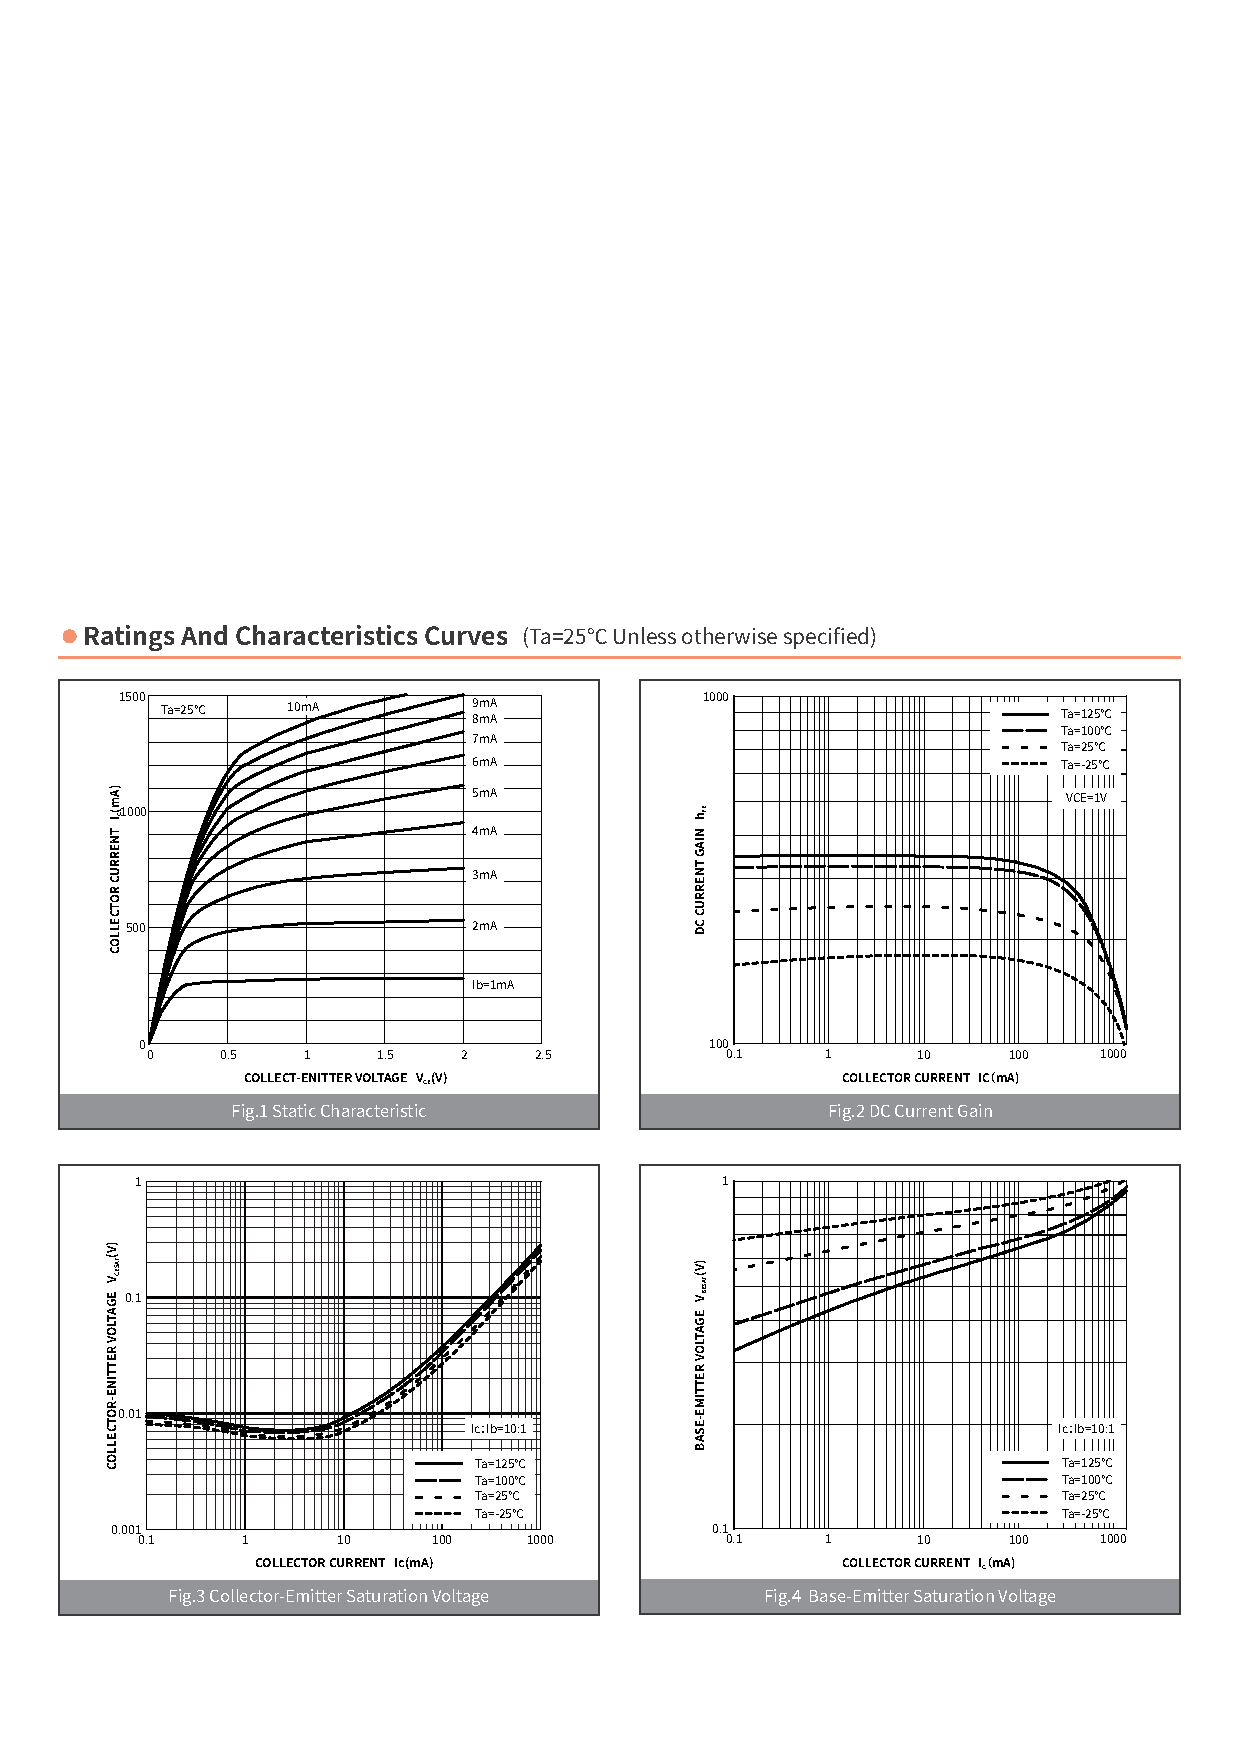
\includegraphics[width=\columnwidth]{preview/assets/SS8050_3.pdf}
\end{figure}

\section{Technical Parameters of The Oscilloscope and The Multimeter}

我们的示波器测量范围和精度均高于万用表,因此采用示波器进行测量。示波器 (Rigol 200MSO2202A) 的主要参数如下:
\begin{enumerate}
    \item 带宽: 200 MHz
    \item 输入阻抗::(1 MΩ±1\%)||(16 pF±3 pF)或 50 Ω±1.5\%
    \item 时基档位:1.000 ns/div至1.000 ks/div
    \item 时基精度: ≤±25 ppm
    \item 垂直档位:输入阻抗为50 Ω时:500 μV/div至1 V/div
    \item 输入阻抗为1 MΩ时:500 μV/div至10 V/div
    \item 偏移范围:输入阻抗为50 Ω时: 500 μV/div 至 50 mV/div:±2 V ; 51 mV/div至200 mV/div:±10 V ; 205 mV/div 至1 V/div:±12 V
    \item 输入阻抗为1 MΩ时:500 μV/div至50 mV/div:±2 V ; 51 mV/div至200 mV/div:±10 V ; 205 mV/div至2 V/div:±50 V ; 2.05 V/div至10 V/div:±100 V
    \item 直流增益精度:±2\%满刻度
    \item 直流偏移精度:±0.1 div±2 mV±1\%偏移值
\end{enumerate}

\noindent 万用表 (Unit UT61E) 的主要参数如下:
\begin{enumerate}
    \item 精度:AC 电压测量范围: 220mV/2.2V/22V/220V/750V
    \item AC 电压测量精度:±(0.8\% + 10 digit)
    \item AC 电压测量带宽:45Hz-10kHz
    \item AC 电流量程:220μA/2.2mA/22mA/220mA/10A
    \item AC 电流测量准确度:±(0.8\% + 10 digit)
    \item AC 电流测量带宽:45Hz-10kHz
\end{enumerate}

%\section{异常现象分析}


\section{Common-Emitter Amplifier Design}

\begin{figure}[H]\centering
\begin{subfigure}[b]{0.5\columnwidth}\centering
    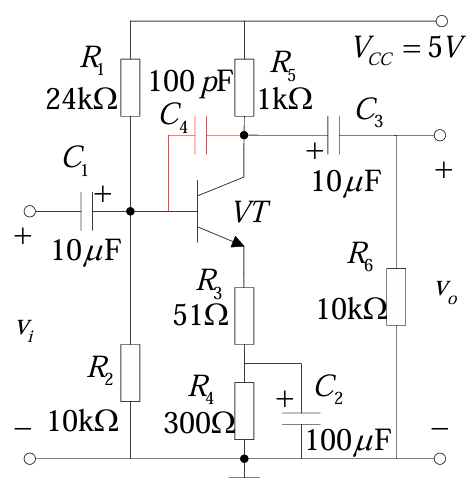
\includegraphics[height=190pt]{preview/assets/CE.png}
    \caption{Circuit Schematic}
\end{subfigure}\hfill
\begin{subfigure}[b]{0.5\columnwidth}\centering
    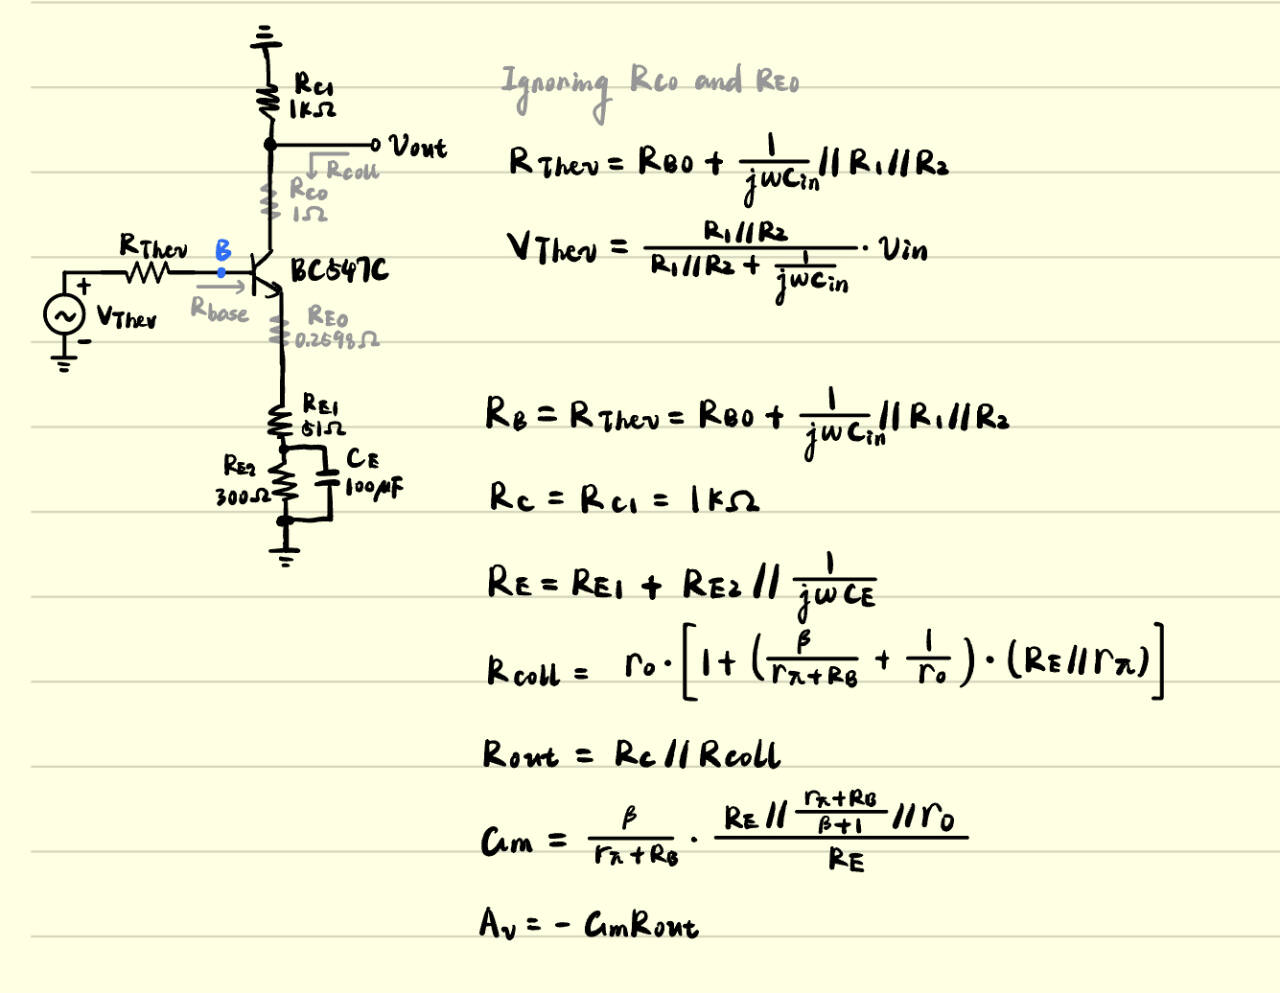
\includegraphics[height=190pt]{preview/assets/Gain.png}
    \caption{Small-Signal (Mid-band) Gain Calculation}
\end{subfigure}
\caption{Design of Common-Emitter Amplifier}
\end{figure}

\section{Input and Output Impedance Calculation}

\noindent 
If considering the coupling capacitors, we have:
\begin{gather}
R_{in} = \frac{1}{j \omega C_1} + R_1 \parallel R_2 \parallel R_{base},\quad 
R_{base} = r_{\pi} + R_E \cdot \frac{\beta r_O + r_O + R_C}{R_E + r_O + R_C}
\\ 
R_{out} = \frac{1}{j \omega C_3} + R_5 \parallel R_{coll},\quad 
R_{coll} = r_O \cdot \left[ 1 + \left(\frac{\beta}{r_{\pi} + R_B} + \frac{1}{r_O}\right)\left(R_E \parallel (r_{\pi} + R_B)\right) \right]
\\
\text{where\ \ }
R_B = R_{Thev} = r_{bb'} + \frac{1}{j \omega C_{1}} \parallel R_1 \parallel R_2
\end{gather}

\noindent 
From another perspective, ignoring the coupling capacitors, we have:
\begin{gather}
R_{in} = R_1 \parallel R_2 \parallel R_{base},\quad 
R_{base} = r_{\pi} + R_E \cdot \frac{\beta r_O + r_O + R_C}{R_E + r_O + R_C}
\\ 
R_{out} = R_5 \parallel R_{coll},\quad 
R_{coll} = r_O \cdot \left[ 1 + \left(\frac{\beta}{r_{\pi} + R_B} + \frac{1}{r_O}\right)\left(R_E \parallel (r_{\pi} + R_B)\right) \right]
\\
\text{where\ \ }
R_B = R_{Thev} = R_{B0} + R_1 \parallel R_2 = r_{bb'}  + R_1 \parallel R_2
\end{gather}
\noindent 
Note that the impedances denote small-signal quantities despite we use the uppercase. For instance, \textbf{ignoring $C_1$ and $C_3$ but considering $C_2$}, and assuming the parameters of the transistor is given by:
\begin{gather}
    I_S = 4.679 \times 10^{-14} \ \mathrm{A}\\
    n_f = 1.01,\ 
    {\color{red} \,\beta = 250\,},\ 
    V_A = 52.64 \ \mathrm{V},\ 
    \\
    R_{B0} = r_{bb'} = 1 \ \Omega,\ 
    R_{E0} = 0.2598 \ \Omega,\ 
    R_{C0} = 1 \ \Omega
\end{gather}
it can be derived that the quiescent operation point is:
\begin{gather}
I_C = 2.178 \ \mathrm{mA},\ 
I_B = 8.712 \ \mathrm{uA}
,\quad 
V_{BE} = 0.644 \ \mathrm{V},\ 
V_{CE} = 2.0547 \ \mathrm{V}
\\
V_E = 0.7651 \ \mathrm{V},\quad 
V_B = 1.4091 \ \mathrm{V},\quad 
V_C = 2.8198 \ \mathrm{V}
\end{gather}
Therefore, the small-signal gain and other parameters is given by (calculated at 1kHz):
\begin{gather}
A_v = -15.6618 - 0.4088j \overset{\mathrm{abs}}{\ =\ } -15.6671,\quad |R_{in}| = 4.8297 \ \mathrm{k}\Omega,\quad |R_{out}| = 992.0509 \ \Omega
\end{gather}

\section{Input/Output Impedance Measurement}

\noindent 
Assuming the open-circuit voltage gain is $A_{0}$, the input source resistance is $R_S$, we have:
\begin{gather}
A_v = \frac{R_{in}}{R_{in} + R_S} A_{0} \Longrightarrow 
R_{in} =  \frac{R_S}{\frac{A_0}{A_v} - 1} \quad (R_L = \infty)
\\ 
A_v = \frac{R_{L}}{R_{L} + R_{out}} A_{0} \Longrightarrow 
R_{out} = \left(\frac{A_0}{A_v} - 1\right) R_L \quad (R_S = 0)
\end{gather}












\section*{Appendix: Matlab Codes of OP, Gain and Impedance Calculation}
\addcontentsline{toc}{section}{附录 \hspace*{6pt} Matlab Codes} 
\thispagestyle{fancy} 
\lstinputlisting{D:/a_RemoteRepo/GH.MatlabCodes/本科课程代码/Linear Circuit Experiment/midterm experiment - common emitter amplifier (20250329).m}





































\end{document}

% VScode 常用快捷键:

% F2:                       变量重命名
% Ctrl + Enter:             行中换行
% Alt + up/down:            上下移行
% 鼠标中键 + 移动:           快速多光标
% Shift + Alt + up/down:    上下复制
% Ctrl + left/right:        左右跳单词
% Ctrl + Backspace/Delete:  左右删单词    
% Shift + Delete:           删除此行
% Ctrl + J:                 打开 VScode 下栏(输出栏)
% Ctrl + B:                 打开 VScode 左栏(目录栏)
% Ctrl + `:                 打开 VScode 终端栏
% Ctrl + 0:                 定位文件
% Ctrl + Tab:               切换已打开的文件(切标签)
% Ctrl + Shift + P:         打开全局命令(设置)

% Latex 常用快捷键:

% Ctrl + Alt + J:           由代码定位到PDF


